\subsection{Sexto \textit{Sprint Huddle} de Producción}
En este sprint se definieron las nuevas estrategias a seguir para agilizar y 
optimizar el desarrollo del juego y el desarrollo de los \textit{sprites} 
faltantes del juego.

\subsubsection{Las nuevas estrategias de desarrollo}
Para el sexto \textit{sprint} y teniendo como base la experiencia de desarrollo los 
anteriores prototipos, quedaba claro que se necesitaba diseñar una nueva estrategia 
que permitiera agilizar el desarrollo del juego sin comprometer la calidad del 
mismo. La naturaleza iterativa de \textit{Huddle} permite controlar la extensión del 
desarrollo y la asignación de tareas entre miembros del equipo, pero al estar 
orientada a niveles producía que la programación se tuviera que pausar cada vez 
que se iniciaba un nuevo nivel para diseñar la maqueta del nivel y para el 
desarrollo de los \textit{sprites}. Por tal motivo se propuso un nuevo enfoque a 
\textit{Huddle} 
orientar su naturaleza iterativa al desarrollo de los componentes del juego, 
una vez que estos esten completados y probado su funcionamiento de manera 
individual, se inicia la construcción de los niveles. Bajo este nuevo enfoque 
primeramente se crean las maquetas de todos los niveles, seguido de la creación 
de todos los \textit{sprites}, para después programar los assets que correspondían a 
los actores, después se implementan las clases controladoras que comparten todos 
los niveles, como el controlador del personaje, el controlador de la barra de vida, 
etc.; con los controladores comunes funcionando se crea una escena base que incluye 
el personaje jugable y la interfaz de juego, sobre esta escena se construyen los 
niveles del juego. El anterior enfoque es una pequeña abstracción del Método \textit{Centry} descrito en la sección \ref{MetodoCerny}.
\\
\par
Ya definido el nuevo plan de trabajo, se procedió a diseñar las maquetas para los 
niveles. Para el diseño de maquetas se siguió utilizando la plantilla creada 
durante Trabajo Terminal 1. Si se desea ver las maquetas de los niveles, estas se 
encuentran en el anexo \ref{MaquetasNiveles}. 
\\
\par
\subsubsection{Actualizando el \textit{software} de desarrollo}
Paralelamente al diseño de las maquetas de los niveles, fue liberada la versión 
2017.3.1f de \textit{Unity3D}. Esta versión incluye herramientas que agilizan la 
creación de niveles como el uso de: 
	\begin{itemize}
		\item \textbf{\textit{Tilemap}:} Herramienta para el mapeado de niveles. Esta 
		herramienta facilita la creación de mapas al crear una malla sobre la que 
		se arrastraran diferentes \textit{Sprites} que se hayan importado previamente 
		al tilemap (ver figura \ref{fig:TilemapPantalla}). En la sección () se 
		profundizará su funcionamiento.
		
		\begin{figure}[h]
    			\centering
    			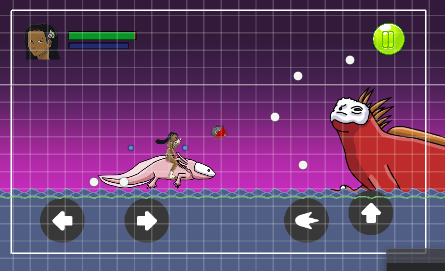
\includegraphics[width=0.6\textwidth]{05TrabajoReali/imagenes/tilemaps01.png}
    			\caption{Vista de la escena cuando se tiene un \textit{GameObject} de 
    			tipo \textit{Tilemaps} para la construcción de niveles}
    			\label{fig:TilemapPantalla}
			\end{figure}
		
		\item \textbf{\textit{Cinemachine}:} \textit{Asset} que permite controlar la 
		cámara de la escena, con este \textit{asset} se le puede indicar que objeto se 
		desea que la cámara siga y se puede asignar un área que limitara el movimiento 
		de la cámara (ver figura \ref{fig:CinemaPantalla}). \textit{Cinemachine} se 
		descarga directamente desde la tienda de \textit{assets} de \textit{Unity} y 
		fue desarrollado por los ingenieros de \textit{Unity}, lo que significa que 
		no genera conflictos o no requiere de configuraciones extras al proyecto para 
		importar. En la sección () se profundizará su funcionamiento.
			
			\begin{figure}[h]
    			\centering
    			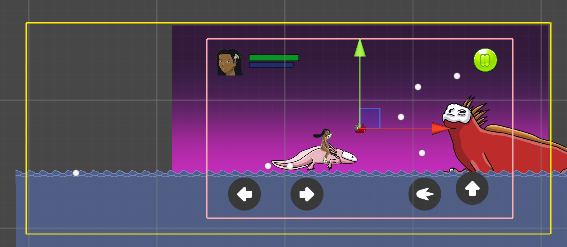
\includegraphics[width=0.6\textwidth]{05TrabajoReali/imagenes/cinemachine01.png}
    			\caption{Vista de la escena cuando se tiene un \textit{GameObject} de 
    			tipo \textit{Tilemaps} para la construcción de niveles}
    			\label{fig:CinemaPantalla}
			\end{figure}

		\item \textbf{\textit{Sprite Packer}}: Si bien no es una herramienta para 
		construcción de niveles o un \textit{asset}, esta herramienta es una de las 
		más útiles que se agregó a la nueva versión de \textit{Unity} ya que, como 
		su nombre lo indica, permite el empaquetado de \textit{sprites} (ver figura ). 
		Empaquetar 
		los \textit{sprites} es una práctica que optimiza el renderizado de objetos, 
		ya que el controlador de gráficos de \textit{Unity} realiza una sola llamada 
		por paquete cuando renderiza los objetos y con esa única llamada renderiza todos 
		los objetos de la escena que se encuentren en ese paquete; si los 
		\textit{sprites} no se encontraran dentro de un paquete el controlador de 
		gráficos de \textit{Unity} haría una llamada por cada \textit{sprite}.  
			\begin{figure}[h]
    			\centering
    			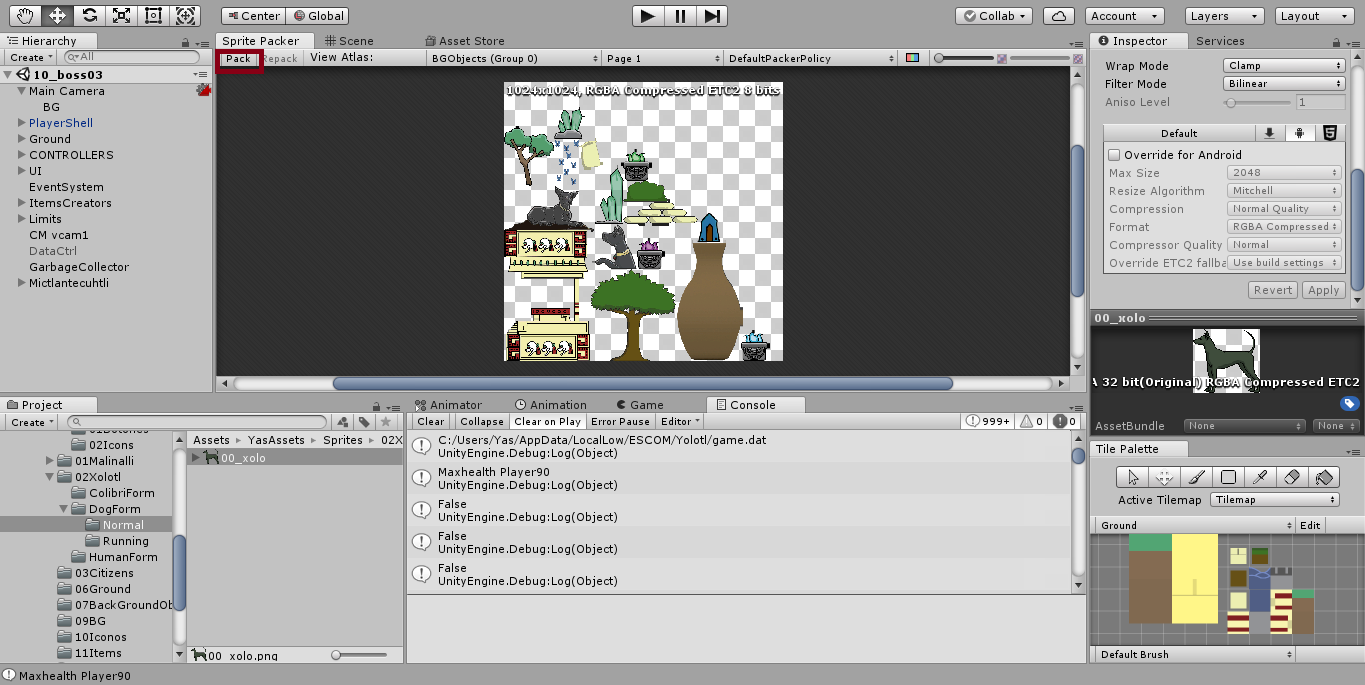
\includegraphics[width=0.6\textwidth]{05TrabajoReali/imagenes/01.png}
    			\caption{Vista de la pestaña del \textit{Sprite Packer}.}
    			\label{fig:CinemaPantalla}
			\end{figure}
	\end{itemize}
	Por el impacto que tendrían las nuevas herramientas de la versión de 
	\textit{Unity}, se propusó utilizarla en lugar de la versión 5.6.2f1. Antes 
	de actualizar la versión de \textit{Unity} se investigó si el proyecto sufriría 
	algún impacto negativo como falta de compatibilidad de componentes por la 
	diferencia de versiones. Al comprobar que existía una total compatibilidad 
	entre ambas versiones en cuanto a trasladar un proyecto de la versión 5.6.1f 
	a la versión 2017.3.1f. Se determinó que la nueva versión de \textit{Unity} 
	sería la que se emplearía para el resto del desarrollo del juego.

\subsubsection{Creación de los \textit{sprites} faltantes}
Lo siguiente a realizarse durante el sexto \textit{sprint} fueron los \textit{sprites}, 
durante las modificaciones que se definieron en Trabajo Terminal 1 fue la 
utilización de un \textit{software} de animación en dos dimensiones para generar 
los \textit{sprites} restantes; sin embargo, el cambio de \textit{software} para 
generar los sprites fue descartado, esto debido a que se adquirió una nueva 
tableta digitalizadora que agilizó la creación de \textit{sprites}. Para Trabajo 
Terminal 2 se dibujaron y digitalizaron más de 100 \textit{sprites}. Para mejorar 
la experiencia visual del jugador se animaron \textit{sprites} que en los primeros 
demos eran estáticos como es el caso de los fantasmas del segundo nivel de la 
sección de plataformas (ver figura \ref{fig:FantasmaAnimacion}). 

%%
\begin{figure}[h]
	\centering
	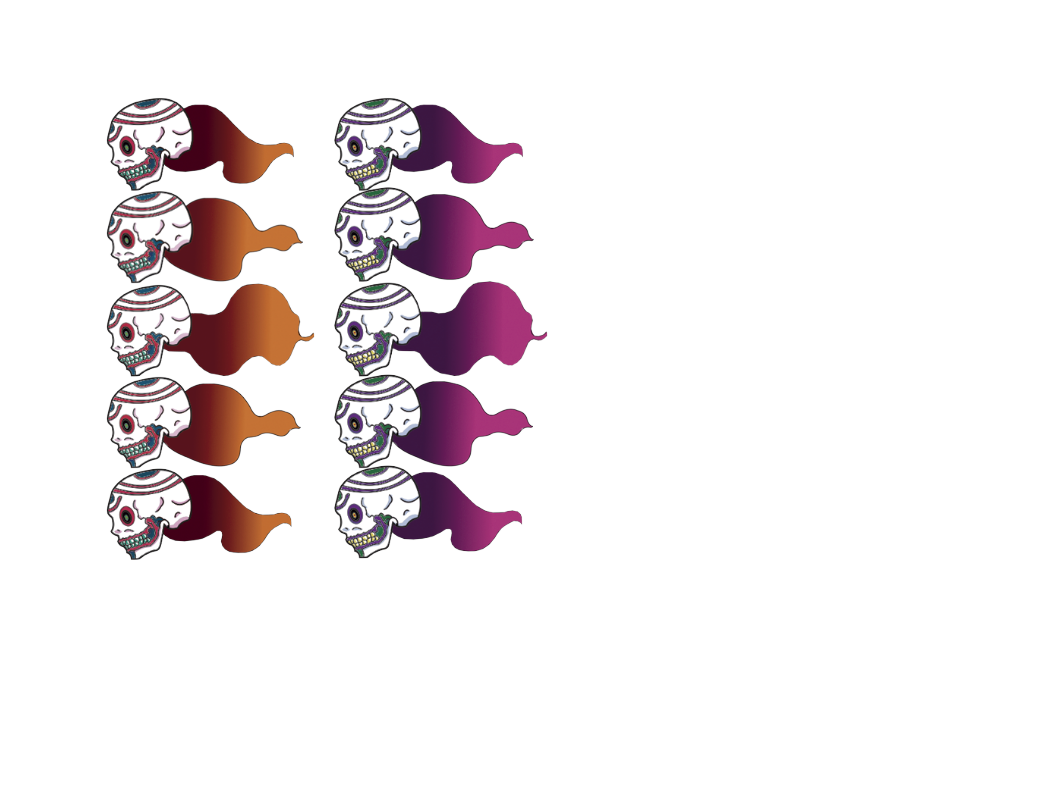
\includegraphics[width=0.4\textwidth]{05TrabajoReali/imagenes/fantasmas.png}
 	\caption{Bloques de animación para el enemigo de tipo fantasma.}
	\label{fig:FantasmaAnimacion}		
\end{figure}

Otros cambios en cuanto el aspecto visual del juego fue la integración de nuevos 
\textit{sprites} para el personaje jugable, los nuevos sprites incluyen la 
caracola que \textit{Malinalli} (ver figura \ref{fig:MalinalliCaracola}) emplea 
para atacar y que se obtiene al final del primer nivel de la sección de selva, 
estos \textit{sprites} para \textit{Malinalli} son utilizados únicamente en los 
niveles posteriores al primer nivel para darle sentido a la narrativa; para el 
segundo nivel se hizo algo parecido, los \textit{sprites} del personaje jugable 
fueron sustituidos por \textit{Malinalli} montando un ajolote (ver figura 
\ref{fig:MalinalliAjolote}), este cambio se hizo para que lo que el jugador vea 
dentro del nivel sea coherente con la narrativa propuesta y se mejore la inmersión del juego. 

\begin{figure}[h]
	\centering
	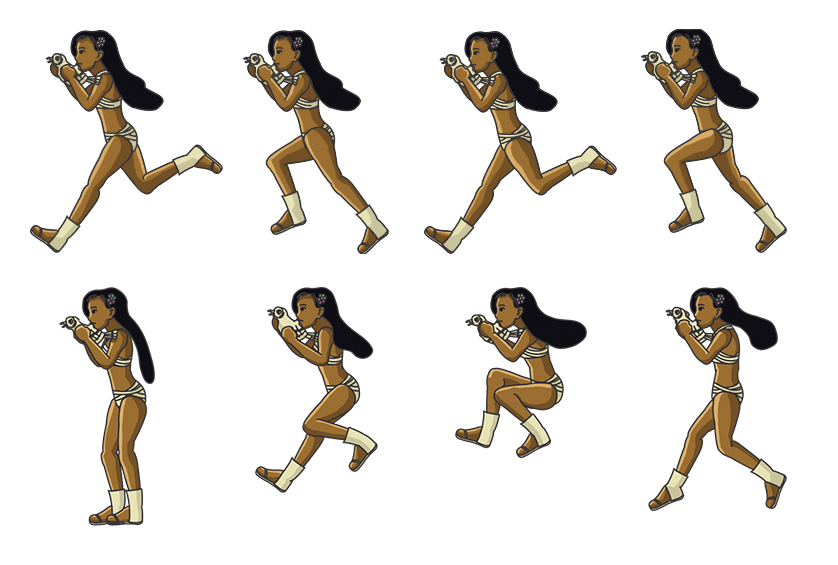
\includegraphics[width=0.4\textwidth]{05TrabajoReali/imagenes/MalinalliArma.png}
 	\caption{Bloques de animación para \textit{Malinalli} posterior a que ella obtiene la caracola.}
	\label{fig:MalinalliCaracola}		
\end{figure}

\begin{figure}[h]
	\centering
	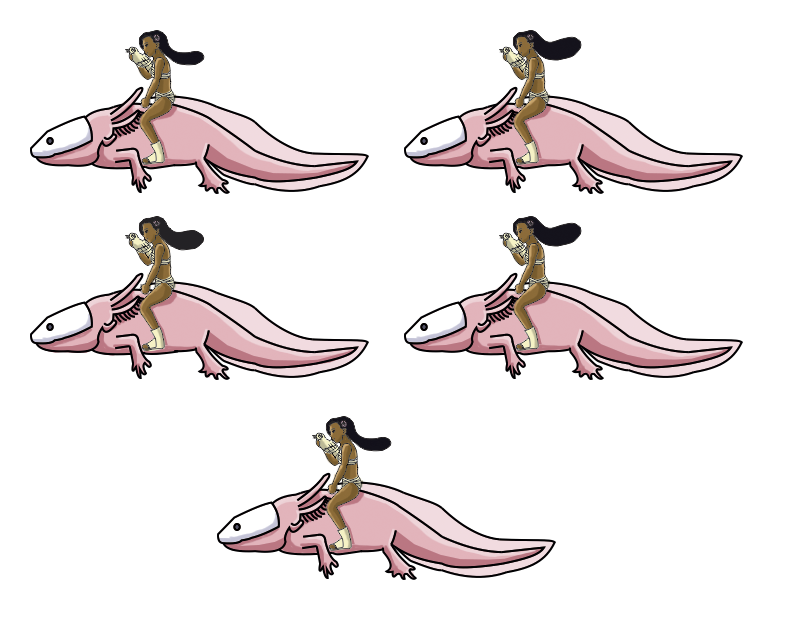
\includegraphics[width=0.5\textwidth]{05TrabajoReali/imagenes/MalinaliAjolote.png}
 	\caption{Bloques de animación para \textit{Malinalli} montando al ajolote del segundo nivel del juego.}
	\label{fig:MalinalliAjolote}		
\end{figure}

En lo que se refiere a los Jefes de cada nivel, no solo se crearon sus respectivos \textit{sprites}, también fue necesario la creación de los \textit{sprites} referentes a sus ataques, para el caso particular de \textit{Mictlantecuhtli} se dibujaron 30 \textit{sprites} tanto para la animación del personaje como para la animación de sus respectivos ataque (ver figura \ref{fig:Mictlantecutli}). Para el diseño de la interfaz gráfica de usuario(\textit{GUI} por sus siglas en íngles) se emplearon \textit{sprites} de las paginas \textit{Kenney.nl} y \textit{Game Art 2D}. Es importante aclarar que la creación de \textit{sprites} pudo haber sido sustituida utilizando paquetes de \textit{sprites} que existen en la red y que son de licencia libre; sin embargo, con la creación de \textit{sprites} propios para el juego se consigue crearle una identidad visual propia al juego, esto permite que el jugador se identifique con mayor facilidad con el personaje y tenga una mejor asociación con el mundo y la historia que se le presenta dentro del juego [cita]. Si se desea ver a profundidad los {sprites} que se crearon se puede consultar el anexo \ref{Anexo:Personajes}. 


\begin{figure}[h]
	\centering
	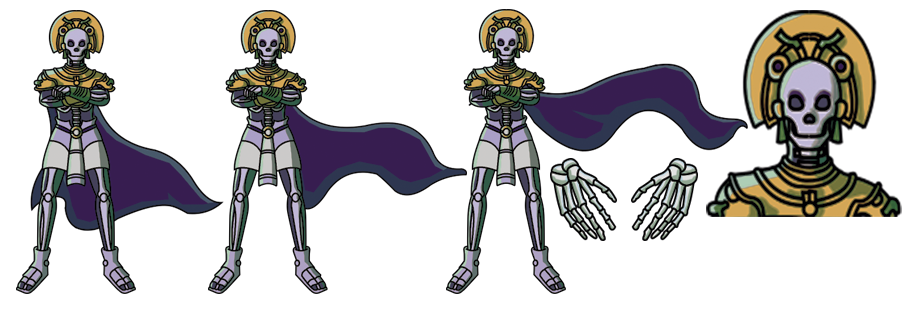
\includegraphics[width=0.5\textwidth]{05TrabajoReali/imagenes/Mictlantecuhtli.png}
 	\caption{Bloques de animación para \textit{Mictlantecuhtli}, jefe final del juego.}
	\label{fig:Mictlantecutli}		
\end{figure}
